\subsection{Ajuste de dos conjuntos de parámetros DFTB}

Como fue introducido en la sección \ref{s:dftb}, para el método DFTB hay dos 
grupos de parámetros a ser determinados, los electrónicos (los orbitales 
pseudoatómicos y las densidades electrónicas) y los potenciales repulsivos para 
cada par de elementos químicos (Si-Si, Si-Li y Li-Li). La optimización de cada 
uno de ellos está sujeta a reproducir alguna propiedad deseada, como la 
estructura de bandas, las energías de atomización, entre otras. Para el ajuste
de la estructura de bandas se siguió el trabajo de van den Bossche \cite{van2019},
considerándose para el Li los electrones de valencia 2s mientras que para el Si 
los 3s y los 3p. La comparación de la estructura de bandas entre DFTB y DFT para 
los conjuntos A y B de parámetros se analiza en profundidad en la referencia 
\cite{oviedo2023}.
%\begin{figure}[th]
%    \centering
%    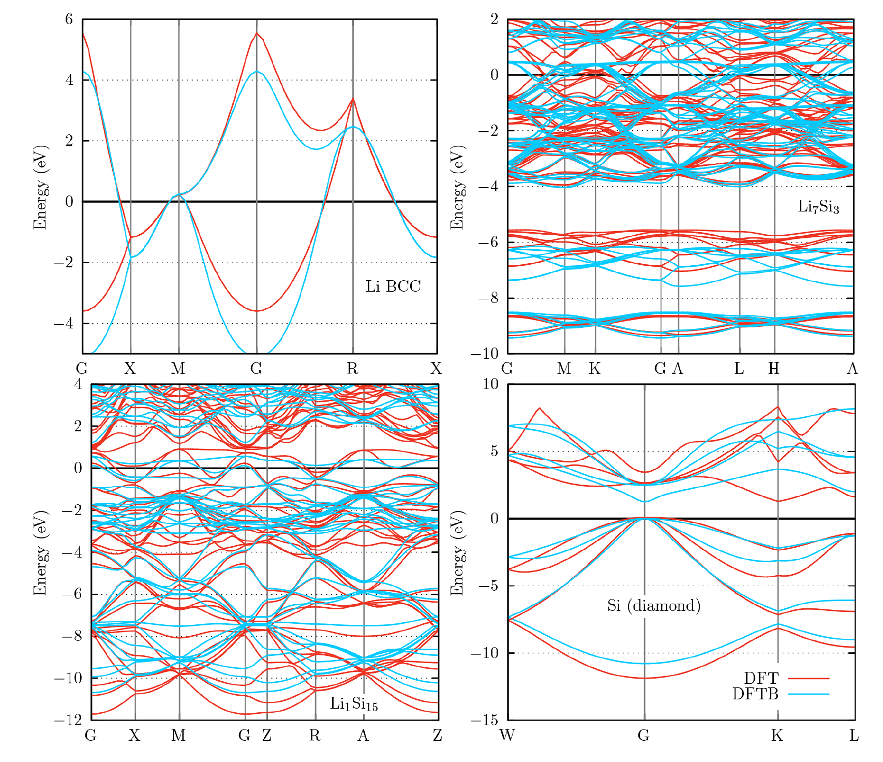
\includegraphics[width=\textwidth]{Silicio/modelo/resultados/bandas/bandas.png}
%    \caption{Estructuras de banda calculadas por DFTB utilizando los dos conjuntos
%    A y B de parámetros, en comparación con las estructuras de banda calculadas 
%    por DFT/PBE para Li (bcc), Li$_7$Si$_3$, Li$_1$Si$_{15}$, y Si (diamante). 
%    Todas las bandas electrónicas están desplazadas a los niveles de Fermi (0 eV)
%    respectivos.}
%    \label{fig:bandas}
%\end{figure}

Para la parametrización del potencial de repulsión de cada uno de los conjuntos 
A y B se siguió el algoritmo de ajuste descripto en la sección \ref{s:algfit}
que permite optimizar los pesos de cada una de las estructuras en el conjunto de 
entrenamiento. Los coeficientes $\check{\boldsymbol{\xi}}_s$ minimizados para cada
conjunto, A y B, se reportan en la Tabla \ref{t:xiweights}.
\begin{table}[b]
    \centering
    \caption{Pesos óptimos, $\check{\boldsymbol{\xi}}_s$, de cada conjunto.}
    \setlength\extrarowheight{2pt}\stackon{%
    \begin{tabular}{l c c}
        \toprule
        \textbf{$s$} & 
        \textbf{conjunto A} & 
        \textbf{conjunto B} \\ 
        \midrule
        Li & $0.23\times10^{-2}$ & 0.49 \\
        Li$_{15}$Si$_4$ & 0.15 & 0.28$\times10^{-21}$ \\
        Li$_{13}$Si$_4$ & 0.21 & 0.17$\times10^{-1}$ \\
        Li$_7$Si$_3$ & 0.21 & 0.11$\times10^{-1}$ \\
        Li$_{12}$Si$_7$ & 0.23 & 0.11$\times10^{-2}$ \\
        LiSi & 0.21 & 0.35$\times10^{-3}$ \\
        Si & 0.83$\times10^{-7}$ & 0.49 \\
        \bottomrule
    \end{tabular}
    }{}
    \label{t:xiweights}
\end{table}
Es interesante que para el conjunto A el algoritmo reduce los pesos relativos del 
Li y del Si puro y aumenta los de las aleaciones. Mientras que para el conjunto 
B sucede lo contrario, los pesos óptimos son mayores para los elementos puros y
menores para las aleaciones. Este comportamiento se debe a que el término de la 
energía de bandas del conjunto A se construye utilizando los elementos puros 
mientras que el mismo término para el conjunto B utiliza una de las aleaciones. 
Resulta razonable que el término de repulsión, que busca compensar el residuo de la 
energía dada por todas las demás contribuciones energéticas, sea menos importante 
para las estructuras consideradas en el ajuste de las energías de banda y más 
importante para el resto. Así, los coeficientes óptimos $\check{\boldsymbol{\xi}}_s$ 
parecen ser capaces de percibir esta situación y tratar de compensarla al centrar 
la parametrización en las estructuras que más la necesitan.

Otra observación que surge de la Tabla \ref{t:xiweights} es el peso relativo bajo
que resulta en ambos conjuntos para la aleación cristalina Li$_{15}$Si$_4$, en 
comparación con el resto de las aleaciones. En particular, para el conjunto B este 
peso es prácticamente igual a cero, indicando que la inclusión de estas 
estructuras en el conjunto de entrenamiento no contribuye a una mejora de la 
predicción de las energías de formación relativas. Esto puede deberse a que la 
estructura de Li$_{15}$Si$_4$ tiene una naturaleza particular que difiere del 
resto de las aleaciones e interfiere de alguna manera con el ajuste de los 
parámetros del modelo. Por ejemplo, una explicación posible puede ser que el 
entorno químico de esta estructura es bastante diferente al del resto de las 
aleaciones por lo que la predicción global puede ser mejorada al centrar el 
ajuste en el resto de las aleaciones. En este sentido, el procedimiento de 
optimización propuesto en este capítulo puede considerarse como una herramienta 
para detectar peculiaridades dentro del conjunto de entrenamiento.
